\documentclass{anstrans}
%%%%%%%%%%%%%%%%%%%%%%%%%%%%%%%%%%%
\title{A Simple Reactor-Model Game to Assist Conceptual Learning}
\author{Robert W.~Carlsen,$^{*}$ Matthew J.~Gidden$^{\*}$}

\institute{
$^{*}$University of Wisconsin, Nuclear Engineering Dept., 1500 Engineering Dr., Madison, WI
}

\email{rcarlsen@wisc.edu \and gidden@wisc.edu}

%%%% packages and definitions (optional)
\usepackage{graphicx} % allows inclusion of graphics
\usepackage{booktabs} % nice rules (thick lines) for tables
\usepackage{microtype} % improves typography for PDF

\usepackage{url}

\newcommand{\SN}{S$_N$}
\renewcommand{\vec}[1]{\bm{#1}} %vector is bold italic
\newcommand{\vd}{\bm{\cdot}} % slightly bold vector dot
\newcommand{\grad}{\vec{\nabla}} % gradient
\newcommand{\ud}{\mathop{}\!\mathrm{d}} % upright derivative symbol

\begin{document}
%%%%%%%%%%%%%%%%%%%%%%%%%%%%%%%%%%%%%%%%%%%%%%%%%%%%%%%%%%%%%%%%%%%%%%%%%%%%%%%%
\section{Introduction}

Engineering learning and teaching styles are known to be somewhat contradictory
\cite{felder2000learning}. While many students tend to prefer active and visual
learning, most education is in the form of abstract and sequential
concepts. This is no different in nuclear engineering, where complicated
concepts such as energy and direction-dependent, neutron transport are
transmitted. Computer games provide a fun and natural way to reinforce learning
and gain valuable intuition for physical phenomena. In this vein, an open-source,
neutron-physics simulation game was created that allows users to explore
interactions of neutrons with different materials and geometric
configurations. Basic concepts such as scattering, absorption, fission are
exposed to students in an interactive, composible environment. Used in
conjunction with traditional teaching methods, such a tool may prove valueable
in an effort to instill basic physical intuition and accelerate the learning of
such complicated subject matter.

%%%%%%%%%%%%%%%%%%%%%%%%%%%%%%%%%%%%%%%%%%%%%%%%%%%%%%%%%%%%%%%%%%%%%%%%%%%%%%%%
\section{Methodology}

On each time step of the simulation, neutron positions are updated as a
function of their velocities.  Then, if the neutron is inside any material,
possible reactions (e.g. fission, scattering, etc.) occur according to
probabilities defined by that material.  These probabilities are calculated as
a function of distance each neutron traveled on the current time step.
Physics concepts modeled include:

\begin{itemize}

    \item Absorption: The probability of absorption is a function of neutron
        energy/speed.  Absorber material can also be burned up over time.

    \item Scattering: All scattering is isotropic.

    \item Fission: The probability of fission is a function of neutron
        energy/speed.  Fuel material can also be burned up over time, loosing
        reactivity.

    \item Moderation: Neutrons can loose some portion of their energy when
        scattering in certain materials. Some materials moderate more or less
        effectively as a function of their "temperature" (number of neutrons
        inside them) - this enables crude modeling of concepts like reactor
        void coefficients.

\end{itemize}

In addition to the neutron population, the positions of materials and other
blocks are tracked and drawn to the screen in real-time.  The user can drag
around material blocks with the mouse.  Partially transparent detector blocks
can also be moved around by the user to investigate neutron populations of
specific parts of the simulation environment.  The user can also introduce
isotropic bursts of neutrons at any location they right-click in the
environment (including inside material blocks).

There are many improvements and features waiting to be added.  One limitation
involves how time steps are calculated.  Because the simulation operates with
a variable frame rate, the time change and position change for neutrons
between time steps increases as the system becomes more computationally
expensive to model (i.e. too many neutrons on the screen).  This slowdown
results in neutrons traveling too far between events and reaction
probabilities being scaled inappropriately high.  This could be prevented by
adjusting a neutron weight parameter instead of increasing the neutron
population when the time change between time steps grows too large.  This
would simulataneously allow the user to see how power continues to grow over
much longer periods of time in supercritical configurations.  

%%%%%%%%%%%%%%%%%%%%%%%%%%%%%%%%%%%%%%%%%%%%%%%%%%%%%%%%%%%%%%%%%%%%%%%%%%%%%%%%
\section{Experiments and Results}

Below, three simple experiments are presented that show how this simulation
game can be used to explore nuclear engineering principles.  Because this
simulation game is open source, you can download and run these (and other)
experiments yourself.  The code is available on Github at
\url{https://github.com/rwcarlsen/reactor}.  Materials and other objects used
in the simulation experiments below are represented by different colored
squares.  The meaning of each square is as follows:

\begin{itemize}
        
    \item White (large): neutron energy independent scattering medium.

    \item Green (medium): neutron energy independent moderating/scattering.
        medium.

    \item Blue (medium): neutron energy dependent burnable absorber.

    \item Purple (small): fissile material or fuel.

    \item Olive (small): togglable constant streaming neutron source.

    \item Yellow (transparent): neutron detector that reports the number of
        neutrons inside it without affecting neutrons or material properties
        underneath itself.

\end{itemize}


\subsection{Attenuation}

\begin{figure}
    \centering
    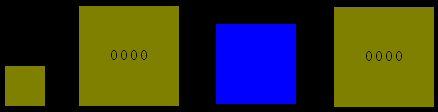
\includegraphics[width=\columnwidth]{atten-setup.png}
    \caption{An attenuation experiment with a directable beam neutron source,
      detector, absorbing material, and an additional detector.}
    \label{fig:atten-setup}
\end{figure}

\begin{figure}
    \centering
    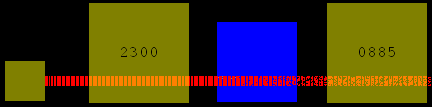
\includegraphics[width=\columnwidth]{atten-on.png}
    \caption{Initially, attenuation is shown due to neutron absorption.}
    \label{fig:atten-on}
\end{figure}

\begin{figure}
    \centering
    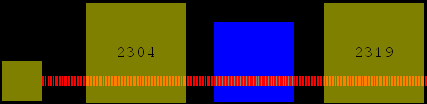
\includegraphics[width=\columnwidth]{atten-done.png}
    \caption{Upon depeletion of the absorber, no attenuation of neutrons is observed.}
    \label{fig:atten-done}
\end{figure}

\begin{figure}
    \centering
    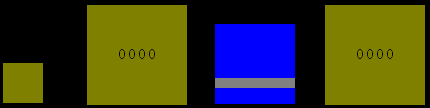
\includegraphics[width=\columnwidth]{atten-off.png}
    \caption{After turning off the neutron beam, absorber depletion is observable.}
    \label{fig:atten-off}
\end{figure}

\subsection{Criticality and Burnup}

\begin{figure}
    \centering
    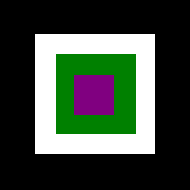
\includegraphics{reactor-thermal-setup.png}
    \caption{Supercritical thermal reactor setup.}
    \label{fig:thermal-setup}
\end{figure}

\begin{figure}
    \centering
    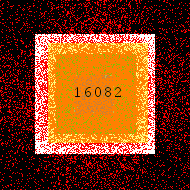
\includegraphics{reactor-thermal-1min.png}
    \caption{Supercritical thermal reactor continues to grow its neutron population. }
    \label{fig:thermal-on}
\end{figure}

\begin{figure}
    \centering
    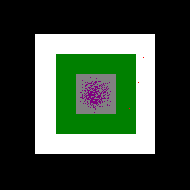
\includegraphics{reactor-thermal-after.png}
    \caption{After shutdown, the thermal reactor exhibits non-uniform burnup in the fuel. }
    \label{fig:thermal-after}
\end{figure}

\subsection{Subcritical Multiplication}

\begin{figure}
    \centering
    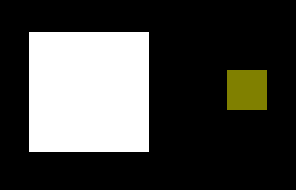
\includegraphics{scatter-setup.png}
    \caption{Reference setup for measuring neutron equilibrium in a scattering medium.}
    \label{fig:scatter-setup}
\end{figure}

\begin{figure}
    \centering
    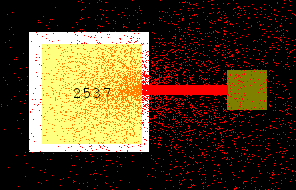
\includegraphics{scatter-equil.png}
    \caption{Reference scattering setup reaches an equilibrium neutron population of about 2500 neutrons when fed by a constant streaming source.}
    \label{fig:scatter-equil}
\end{figure}

\begin{figure}
    \centering
    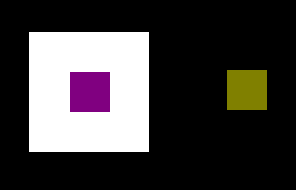
\includegraphics{subcrit-mult-setup.png}
    \caption{Fuel was introduced into the scattering medium creating a subcritical multiplication configuration.}
    \label{fig:subcrit-setup}
\end{figure}

\begin{figure}
    \centering
    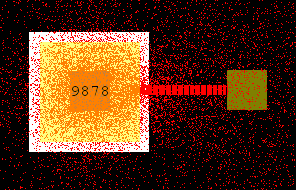
\includegraphics{subcrit-mult-equil.png}
    \caption{Subcritical multiplication reaches an equilibrium neutron population of about 10,000 neutrons when fed by a constant neutron source.}
    \label{fig:subcrit-equil}
\end{figure}

For those who like equations in their papers, \LaTeX\ is a good choice. Here is
an equation for the Marshak diffusion boundary condition:
\begin{equation} \label{eq:marshak}
  4 J^- = \phi + 2 D \vec{n} \vd \grad \phi \,.
\end{equation}
If we so choose, we can effortlessly reference the equation later.

Another paragraph starts with Eq.~\eqref{eq:marshak} and sets $J^-$ to zero, a
vacuum boundary condition:
\begin{equation*}
  0 = \phi + \frac{2}{3} \frac{1}{\sigma} \vec{n} \vd \grad \phi \,.
\end{equation*}

The extrapolation distance is $2/3$. A more detailed asymptotic analysis yields
an extrapolation distance of about $0.71045$.

Later on, we can include a table, even one that spans two columns such as
Table~\ref{tab:widetable}.
%%%%%%%%%%%%%%%%%%%%%%%%%%%%%%%%%%%%%%%%
\begin{table*}[htb]
  \centering
\begin{tabular}{llllllllll}\toprule
      & $\phi_T(0)$      & $\phi_T(10)$      & $\phi_T(20)$      &
      $\phi_D(0)$      & $\phi_D(10)$      & $\phi_D(20)$      & $\rho$      &
      $\varepsilon$      & $N_\text{it}$
\\ \midrule
$c=0.999$  & 0.9038 & 20.63 & 31.24 & 0.9087 & 20.63 & 31.23 & 0.2192 & $10^{-7}$ & 15
\\
$c=0.990$  & 0.3675 & 13.04 & 24.7 & 0.3696 & 13.04 & 24.69 & 0.2184 & $10^{-7}$ & 15
\\
$c=0.900$  & 0.009909 & 4.776 & 17.64 & 0.009984 & 4.786 & 17.63 & 0.2118 & $10^{-7}$ & 14
\\
$c=0.500$  & $6.069\times 10^{-5}$ & 2.212 & 15.53 & 6.213$\times 10^{-5}$ & 2.239 & 15.53 & 0.2068 & $10^{-7}$ & 13
\\
\bottomrule
\end{tabular}
  \caption{This is an example of a really wide table which might not normally
  fit in the document.}
  \label{tab:widetable}
\end{table*}

%%%%%%%%%%%%%%%%%%%%%%%%%%%%%%%%%%%%%%%%%%%%%%%%%%%%%%%%%%%%%%%%%%%%%%%%%%%%%%%%
\section{Conclusions}


This and other limitations could easily be improved upon.  

%%%%%%%%%%%%%%%%%%%%%%%%%%%%%%%%%%%%%%%%%%%%%%%%%%%%%%%%%%%%%%%%%%%%%%%%%%%%%%%%
\section{Acknowledgments}
This material is based upon work supported a Department of Energy Nuclear
Energy University Programs Graduate Fellowship.

%%%%%%%%%%%%%%%%%%%%%%%%%%%%%%%%%%%%%%%%%%%%%%%%%%%%%%%%%%%%%%%%%%%%%%%%%%%%%%%%
\bibliographystyle{ans}
\bibliography{bibliography}
\end{document}

